La arquitectura de \textit{NodeAlert IoT} se fundamenta en un modelo jerárquico y distribuido que separa las tareas de adquisición, gestión de red y servicios de aplicación. Esta estructura, alineada con las arquitecturas modernas de \textit{Internet of Things} (IoT), garantiza que el sistema sea escalable y presente una alta tolerancia a fallos en entornos críticos.

\subsection{Descripción del Ecosistema}
El ecosistema se organiza en tres capas funcionales, permitiendo que cada componente opere con el determinismo requerido para sistemas de tiempo real \citep{valvano2014volume2}:

\begin{enumerate}[label=\alph*)]
    \item \textbf{Capa de Percepción (Nodos ESP32):} Conformada por múltiples nodos basados en el microcontrolador ESP32. Cada nodo actúa como una unidad de procesamiento en el borde (\textit{Edge Node}), encargada de la lectura de sensores ambientales (DHT22, MQ-9, KY-026), la ejecución de lógica de control local inmediata y la activación de un buzzer de alarma ante condiciones peligrosas. Los nodos se conectan directamente al broker MQTT por WiFi sin necesidad de un gateway intermedio.
    \item \textbf{Capa de Servidor (Raspberry Pi):} Una Raspberry Pi ejecuta Docker Compose con cuatro servicios: el broker MQTT Mosquitto para la mensajería asíncrona, el backend Django con MySQL para la persistencia y API REST, el frontend React servido por Nginx, y Nginx como proxy reverso.
    \item \textbf{Capa de Aplicación:} El punto de interacción con el usuario final, compuesto por un \textit{dashboard} web desarrollado en React con Material UI para monitoreo en tiempo real, visualización de gráficos históricos y envío de comandos a los nodos.
\end{enumerate}
\begin{figure}[H]
    \centering
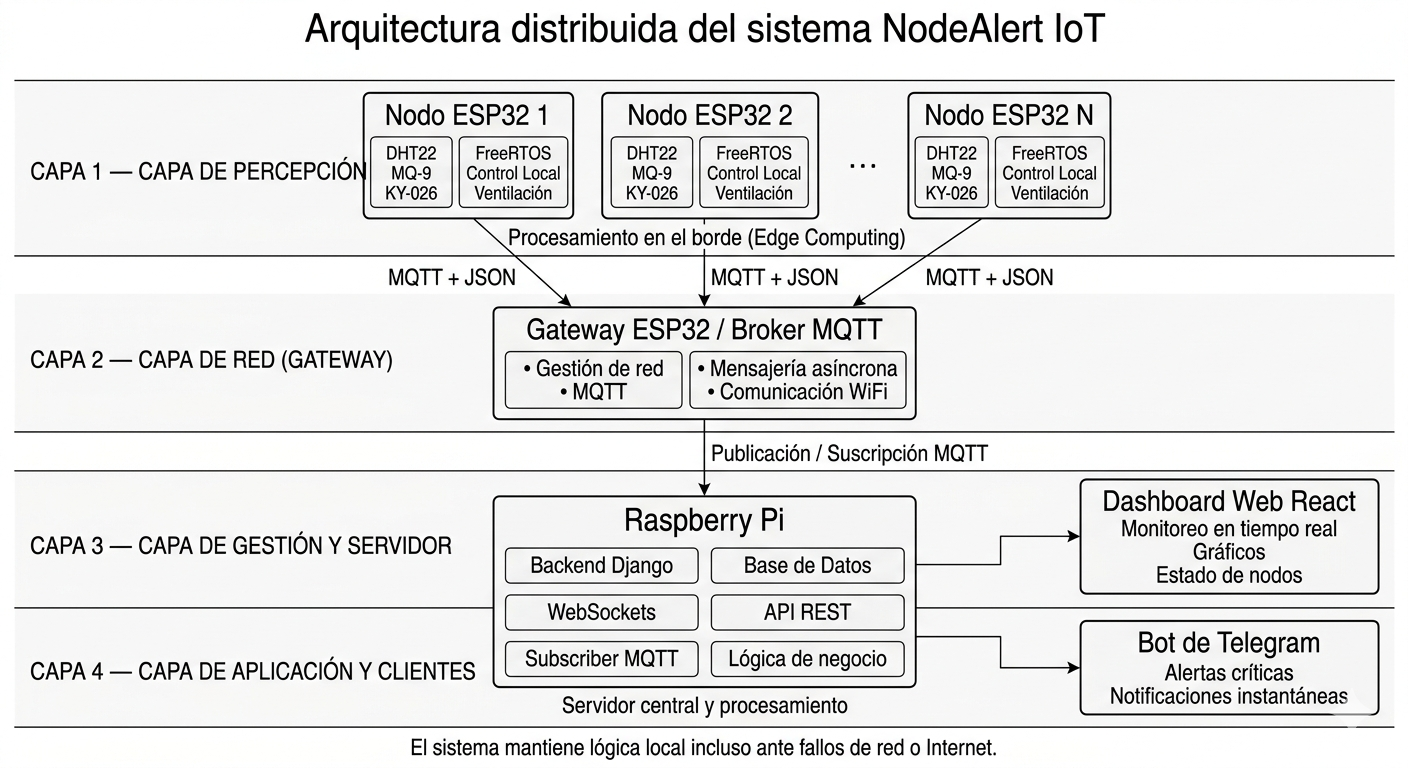
\includegraphics[width=1.1\linewidth]{aqrdistru.png}
    \caption{Arquitectura distribuida del sistema NodeAlert IoT: Interacción entre Nodos ESP32, Raspberry Pi y Cliente Web.}
     \label{fig:arquitectura_general}
 \end{figure}

\subsection{Flujo de Datos y Comunicación}
El flujo de información comienza con la digitalización de señales analógicas en los nodos periféricos, siguiendo los principios de análisis de circuitos de \citet{alexander2006}. Los datos se empaquetan en formato JSON y se publican en tópicos específicos de MQTT. 

La separación de estas capas asegura que, incluso si el servidor central o la conexión a Internet fallan, los nodos individuales mantengan la capacidad de ejecutar acciones preventivas locales, cumpliendo con los requisitos de seguridad descritos por \citet{valvano2014volume1} para sistemas embebidos de misión crítica.

% FOTO REAL: aqrdistru.png